\section{Quantum Systems}

\paragraph{The Idea}
For this consideration of quantum systems, the idea is to have the system interact with some bath containing an enormous number of degrees of freedom relative to those of the system.

\paragraph{The Reduced Density Matrix}
The reduced density matrix is found by tracing out a particular set of degrees of freedom from a total density matrix.

\paragraph{Product Operators}
We recall that for a tensor product, the expectation value of the product is the product of the expectation values. This means that expectation values of system observables make sense.

\paragraph{Schmidt Decomposition}
Consider a system in contact with a bath. A general state can be written as
\begin{align*}
	\ket{\Psi} = \sum\limits_{a}\sum\limits_{\alpha}\Psi_{a\alpha}\ket{a}\otimes\ket{\alpha},
\end{align*}
where the latin and greek indices indicate states in the system and bath respectively. We may equivalently consider a state as specified by a matrix $\Psi$ with elements $\Psi_{a\alpha}$. The singular value decomposition of $\Psi$ is
\begin{align*}
	\Psi = U\Lambda V\adj
\end{align*}
for some set of matrices $U, \Lambda$ and $V$ such that $\Lambda$ is a rectangular diagonal matrix with positive elements and $U$ and $V$ are unitary. We may then write
\begin{align*}
	\Psi_{a\alpha} = \sum\limits_{b}U_{ab}(\Lambda V\adj)_{b\alpha} = \sum\limits_{b}\sum\limits_{\beta}U_{ab}\Lambda_{b\beta}(V\adj)_{\beta\alpha}.
\end{align*}
Because $\Lambda$ is diagonal, summing over $\beta$ only gives a contribution when $b = \beta$, hence
\begin{align*}
	\Psi_{a\alpha} = \sum\limits_{b}U_{ab}\lambda_{b}(V\adj)_{b\alpha},
\end{align*}
and
\begin{align*}
	\ket{\Psi} &= \sum\limits_{a}\sum\limits_{\alpha}\sum\limits_{b}U_{ab}\lambda_{b}(V\adj)_{b\alpha}\ket{a}\otimes\ket{\alpha} \\
	           &= \sum\limits_{b}\lambda_{b}\sum\limits_{a}U_{ab}\ket{a}\otimes\sum\limits_{\alpha}(V\adj)_{b\alpha}\ket{\alpha}.
\end{align*}
Because $U$ and $V$ are unitary, the above product contains two proper states. Naming them $\ket{b}_{\text{S}}$ and $\ket{b}_{\text{B}}$ we have
\begin{align*}
	\ket{\Psi} &= \sum\limits_{b}\lambda_{b}\ket{b}_{\text{S}}\otimes\ket{b}_{\text{B}}.
\end{align*}

One thing that was somewhat brushed over in this treatment is the kind of summation performed in the decomposition. Its limits depend on the structure of $\Psi$. This case is valid for when $\Psi$ has more columns than rows, but if the other were to be the case, we could use a similar treatment to obtain a sum over greek indices instead. The point is that we are summing over the singular values, the number of which is equal to the smaller of the sizes of $\Psi$.

\paragraph{The Schrödinger Langevin Equation}
We will now perform a similar consideration as that done in the classical case, namely extending the Schrödinger equation to
\begin{align*}
	i\dv{t}\ket{\Psi} = (H - iW + i\eta(t)V)\ket{\Psi}.
\end{align*}
$W$ is a Hermitian damping term and $\eta$ is a random process such that
\begin{align*}
	\expval{\expval{\eta(t)}} = 1,\ \expval{\expval{\eta(t)\eta\cc(t\p)}} = \delta(t - t\p),
\end{align*}
where we are now referring to averages over the random process rather than quantum mechanical expectation values. This term then corresponds to a noise term. A time step $\delta t$ yields
\begin{align*}
	\ket{\Psi}_{t + \delta t} = \left(1 - (iH + W)\delta t + \integ{t}{t + \delta t}{t\p}{\eta(t\p)V}\right)\ket{\Psi}_{t}.
\end{align*}
Using this we may compute the norm of $\ket{\Psi}$ after this time step according to
\begin{align*}
	\braket{\Psi}_{t + \delta t} =& \expval{\left(1 + (iH - W)\delta t + \integ{t}{t + \delta t}{t\p}{\eta\cc(t\p)V\adj}\right)\left(1 - (iH + W)\delta t + \integ{t}{t + \delta t}{t\p}{\eta(t\p)V}\right)}{\Psi} \\
	                             =& \expval{\left(1 + (iH - W)\delta t\right)\left(1 - (iH + W)\delta t\right)}{\Psi} \\
	                              &+ \expval{\left(1 + (iH - W)\delta t\right)\left(\integ{t}{t + \delta t}{t\p}{\eta(t\p)V}\right)}{\Psi} + \expval{\left(\integ{t}{t + \delta t}{t\p}{\eta\cc(t\p)V\adj}\right)\left(1 - (iH + W)\delta t\right)}{\Psi} \\
	                              &+ \expval{\integ{t}{t + \delta t}{t\p}{\integ{t}{t + \delta t}{t^{\prime\prime}}{\eta(t\p)\eta\cc(t^{\prime\prime})V\adj V}}}{\Psi}.
\end{align*}
Averaging over the random process removes the two terms in the middle. To first order in the time step we therefore have
\begin{align*}
	\braket{\Psi}_{t + \delta t} &= \expval{\left(1 + -2W\delta t\right)}{\Psi} + \expval{\integ{t}{t + \delta t}{t\p}{\integ{t}{t + \delta t}{t^{\prime\prime}}{\delta(t\p - t^{\prime\prime})V\adj V}}}{\Psi} \\
	                             &= \expval{\left(1 - 2W\delta t\right)}{\Psi} + \expval{\integ{t}{t + \delta t}{t\p}{V\adj V}}{\Psi} \\
	                             &= \expval{\left(1 - 2W\delta t\right)}{\Psi} + \delta t\expval{V\adj V}{\Psi},
\end{align*}
and requiring the norm to be preserved by the time step implies
\begin{align*}
	W = \frac{1}{2}V\adj V.
\end{align*}
In summary, the Schrödinger Langevin equation is
\begin{align*}
	i\dv{t}\ket{\Psi} = \left(H - \frac{i}{2}V\adj V + i\eta(t)V\right)\ket{\Psi}.
\end{align*}

\paragraph{The Lindblad Equation}
Using the Schrödinger Langevin equation we may derive a time evolution equation for the density matrix. We have the time evolution operator
\begin{align*}
	U(t, t_{0}) = e^{-i\left(\left(H - \frac{i}{2}V\adj V\right)(t - t_{0}) + i\integ{t_{0}}{t}{t\p}{\eta(t\p)V}\right)},
\end{align*}
and thus
\begin{align*}
	\rho(t) = U(t, t_{0})\rho(t_{0})U\adj(t, t_{0}).
\end{align*}
In particular, for a small time step $\delta t$ we may expand to find
\begin{align*}
	\rho(t + \delta t) =& \left(1 - i\left(\left(H - \frac{i}{2}V\adj V\right)\delta t + i\integ{t}{t + \delta t}{t\p}{\eta(t\p)V}\right)\right)\rho(t)\left(1 + i\left(\left(H + \frac{i}{2}V\adj V\right)\delta t - i\integ{t}{t + \delta t}{t\p}{\eta\cc(t\p)V\adj}\right)\right) \\
	                   =& \rho(t) - i\left(\left(H - \frac{i}{2}V\adj V\right)\delta t + i\integ{t}{t + \delta t}{t\p}{\eta(t\p)V}\right)\rho(t) + i\rho(t)\left(\left(H + \frac{i}{2}V\adj V\right)\delta t - i\integ{t}{t + \delta t}{t\p}{\eta\cc(t\p)V\adj}\right) \\
	                    &+ \integ{t}{t + \delta t}{t\p}{\integ{t}{t + \delta t}{t^{\prime\prime}}{\eta(t\p)\eta\cc(t^{\prime\prime})V\rho(t)V\adj}}.
\end{align*}
Averaging over the noise yields
\begin{align*}
	\rho(t + \delta t) &= \rho(t) - i\left(\left(H - \frac{i}{2}V\adj V\right)\delta t\right)\rho(t) + i\rho(t)\left(\left(H + \frac{i}{2}V\adj V\right)\delta t\right) + \integ{t}{t + \delta t}{t\p}{\integ{t}{t + \delta t}{t^{\prime\prime}}{\delta(t\p - t^{\prime\prime})V\rho(t)V\adj}} \\
	                   &= \rho(t) + i\delta t\left(-\left(H - \frac{i}{2}V\adj V\right)\rho(t) + \rho(t)\left(H + \frac{i}{2}V\adj V\right)\right) + \integ{t}{t + \delta t}{t\p}{V\rho(t)V\adj} \\
	                   &= \rho(t) + \delta t\left(-i\comm{H}{\rho(t)} - \frac{1}{2}\acomm{V\adj V}{\rho(t)} + V\rho(t)V\adj\right),
\end{align*}
and in the limit of infinitesimal time steps we obtain the Lindblad equation
\begin{align*}
	\dv{t}\rho = -i\comm{H}{\rho(t)} - \frac{1}{2}\acomm{V\adj V}{\rho(t)} + V\rho(t)V\adj.
\end{align*}
It may be generalized to a set of interactions with the surroundings by applying a linearity and choosing a basis for the space of operators such that
\begin{align*}
	\dv{t}\rho = -i\comm{H}{\rho(t)} + \sum\limits_{\alpha}V_{\alpha}\rho(t)V_{\alpha}\adj - \frac{1}{2}\acomm{V_{\alpha}\adj V_{\alpha}}{\rho(t)}.
\end{align*}

\paragraph{Third Quantization}
Let $K$ be the space of operators on Hilbert space. Then the Liouville operator
\begin{align*}
	L:\ \rho\to -i\comm{H}{\rho(t)} + \sum\limits_{\alpha}2V_{\alpha}\rho(t)V_{\alpha}\adj - \acomm{V_{\alpha}\adj V_{\alpha}}{\rho(t)},
\end{align*}
which appears in the Lindblad equation (with a different normalization of the jump operators), is a map on $K$. Solving for the dynamics of elements in $K$ is difficult in general, but we will present a way to do it for a particular type of Hamiltonians. This is called third quantization.

A Hamiltonian is quadratic if it is quadratic in creation and annihilation operators. In the case of a non-interacting Hamiltonian, it takes the form
\begin{align*}
	H = \sum\limits_{i, j = 1}^{N}\mqty[
		c_{i}\adj & c_{i}
	]\mqty[
		h_{ij}         & \Delta_{ij} \\
		\Delta_{ij}\cc & h_{ij}\cc
	]\mqty[
		c_{j} \\
		c_{j}\adj
	].
\end{align*}
We rewrite this by introducing creation operators for so-called Majorana fermions
\begin{align*}
	w_{2j - 1} = c_{j} + c_{j}\adj,\ w_{2j} = i(c_{j} - c_{j}\adj),
\end{align*}
of which there are $2N$. We have
\begin{align*}
	w_{2j - 1}\adj = c_{j}\adj + c_{j} = w_{2j - 1},\ w_{2j}\adj = -i(c_{j}\adj - c_{j}) = w_{2j}.
\end{align*}
Assuming the fundamental operators to be fermionic, we have
\begin{align*}
	\acomm{w_{2j - 1}}{w_{2k - 1}} &= \acomm{c_{j} + c_{j}\adj}{c_{k} + c_{k}\adj} \\
	                               &= \acomm{c_{j}}{c_{k}} + \acomm{c_{j}}{c_{k}\adj}+ \acomm{c_{j}\adj}{c_{k}}+ \acomm{c_{j}\adj}{c_{k}\adj} \\
	                               &= 2\delta_{jk}, \\
	\acomm{w_{2j - 1}}{w_{2k}}     &= i\acomm{c_{j} + c_{j}\adj}{c_{k} - c_{k}\adj} \\
	                               &= i\left(\acomm{c_{j}}{c_{k}} - \acomm{c_{j}}{c_{k}\adj} + \acomm{c_{j}\adj}{c_{k}} - \acomm{c_{j}\adj}{c_{k}\adj}\right) \\
	                               &= 0, \\
	\acomm{w_{2j}}{w_{2k}}         &= -\acomm{c_{j} - c_{j}\adj}{c_{k} - c_{k}\adj} \\
	                               &= -\left(\acomm{c_{j}}{c_{k}} - \acomm{c_{j}}{c_{k}\adj} - \acomm{c_{j}\adj}{c_{k}} + \acomm{c_{j}\adj}{c_{k}\adj}\right) \\
	                               &= 2\delta_{jk}.
\end{align*}
We may therefore conclude
\begin{align*}
	\acomm{w_{j}}{w_{k}} = 2\delta_{jk}.
\end{align*}
This implies $w_{i}^{2} = 1$.

Returning to the Hamiltonian, we find that it takes the form
\begin{align*}
	H =& \sum\limits_{i, j = 1}^{N}h_{ij}c_{i}\adj c_{j} + h_{ij}\cc c_{i}c_{j}\adj + \Delta_{ij}c_{i}\adj c_{j}\adj + \Delta_{ij}\cc c_{i}c_{j} \\
	  =& \frac{1}{4}\sum\limits_{i, j = 1}^{N}h_{ij}(w_{2i - 1} + iw_{2i})(w_{2j - 1} - iw_{2j}) + h_{ij}\cc (w_{2i - 1} - iw_{2i})(w_{2j - 1} + iw_{2j})  \\
	   &+ \frac{1}{4}\sum\limits_{i, j = 1}^{N}\Delta_{ij}(w_{2i - 1} + iw_{2i})(w_{2j - 1} + iw_{2j}) + \Delta_{ij}\cc (w_{2i - 1} - iw_{2i})(w_{2j - 1} - iw_{2j}) \\
	  =& \frac{1}{4}\sum\limits_{i, j = 1}^{N}w_{2i - 1}w_{2j - 1}(h_{ij} + h_{ij}\cc + \Delta_{ij} + \Delta_{ij}\cc) + w_{2i - 1}w_{2j}(-ih_{ij} + ih_{ij}\cc + i\Delta_{ij} - \Delta_{ij}\cc)  \\
	   &+ \frac{1}{4}\sum\limits_{i, j = 1}^{N}w_{2i}w_{2j - 1}(ih_{ij} - ih_{ij}\cc + i\Delta_{ij} - i\Delta_{ij}) + w_{2i}w_{2j}(h_{ij} + h_{ij}\cc - \Delta_{ij} - \Delta_{ij}\cc) \\
	  =& \frac{1}{4}\sum\limits_{i, j = 1}^{2N}w_{i}A_{ij}w_{j}
\end{align*}
for some as of yet undetermined matrix $A$. The commutation relations imply
\begin{align*}
	w_{i}A_{ij}w_{j} = 2A_{ij}\delta_{ij} - w_{j}A_{ij}w_{i},
\end{align*}
hence
\begin{align*}
	H &= \frac{1}{8}\sum\limits_{i, j = 1}^{2N}w_{i}A_{ij}w_{j} + 2A_{ij}\delta_{ij} - w_{j}A_{ij}w_{i} \\
	  &= \frac{1}{4}\tr(A) + \frac{1}{8}\sum\limits_{i, j = 1}^{2N}w_{i}A_{ij}w_{j} - w_{j}A_{ij}w_{i} \\
	  &= \frac{1}{4}\tr(A) + \frac{1}{8}\sum\limits_{i, j = 1}^{2N}(A_{ij} - A_{ji})w_{i}w_{j},
\end{align*}
hence we may simplify by redefining $A$. Choosing it to be traceless corresponds to redefining the zero level. We also see that we may choose $A$ to be antisymmetric. Extracting a factor $i$ and choosing $A$ to be real, we find $H$ to be Hermitian, and the final form is
\begin{align*}
	H = \frac{i}{4}\sum\limits_{i, j = 1}^{2N}w_{i}A_{ij}w_{j}.
\end{align*}
We want the Liouvillian to be quadratic as well, hence the jump operators must be of the form
\begin{align*}
	L_{\mu} = \sum\limits_{i}(l_{\mu})_{i}w_{i}.
\end{align*}

On Fock space we construct operators with products of creation and annihilation operators. We want to do the same on $K$, and therefore need a basis on it. We use normal kets to denote elements in $K$, although double wedge brackets are more commonly used. We construct the basis from operator products
\begin{align*}
	w_{1}^{\alpha_{1}}\dots w_{2N}^{\alpha_{2N}},\ \alpha_{i}\in\{0, 1\}.
\end{align*}
The basis is thus comprised of elements
\begin{align*}
	w_{1}^{\alpha_{1}}\otimes w_{2}^{\alpha_{2}}\otimes\dots\otimes w_{2N}^{\alpha_{2N}} = \ket{w_{\vb*{\alpha}}}
\end{align*}
such that
\begin{align*}
	\ket{w_{\vb*{\alpha}}}(w_{\vb*{\alpha}\p}) = \ket{w_{\vb*{\alpha} + \vb*{\alpha}\p\mod 2}},
\end{align*}
where the vector addition is carried out modulo $2$ due to the $w$ squaring to the identity. The dimension of $K$ is identifiable from the above as $D = 2^{2N} = 4^{N}$. We also define the inner product on $K$ as
\begin{align*}
	\braket{x}{y} = \frac{1}{D}\tr(x\adj y),
\end{align*}
where the trace is carried out over $K$. Using this we have
\begin{align*}
	\braket{w_{\vb*{\alpha}}}{w_{\vb*{\alpha}\p}} &= \frac{1}{D}\tr((w_{1}^{\alpha_{1}})\adj (w_{2N}^{\alpha_{2N}})\adj w_{1}^{\alpha_{1}\p}\dots w_{2N}^{\alpha_{2N}\p}) \\
	                                              &= \frac{1}{D}\tr(w_{1}^{\alpha_{1}}w_{1}^{\alpha_{1}\p}\dots w_{2N}^{\alpha_{2N}}w_{2N}^{\alpha_{2N}\p}).
\end{align*}
There are two possibilities. If $\vb*{\alpha} = \vb*{\alpha}\p$ then all operators are merged to form powers of zero or two, and we are left with the trace of the identity, which is equal to $D$. In the other case there exists at least one operator which is not cancelled in the multiplication with the operator. This is equivalent to
\begin{align*}
	\ket{(w_{1}^{\alpha_{1}})\adj (w_{2N}^{\alpha_{2N}})\adj w_{1}^{\alpha_{1}\p}\dots w_{2N}^{\alpha_{2N}\p}}(w_{\vb*{\beta}}) = \ket{w_{\vb*{\gamma}}},\ \vb*{\gamma} \neq \vb*{\beta},
\end{align*}
which implies that $(w_{1}^{\alpha_{1}})\adj (w_{2N}^{\alpha_{2N}})\adj w_{1}^{\alpha_{1}\p}\dots w_{2N}^{\alpha_{2N}\p}$ has no diagonal elements in $K$, and its trace must be zero. In conclusion, we have
\begin{align*}
	\braket{w_{\vb*{\alpha}}}{w_{\vb*{\alpha}\p}} = \delta_{\vb*{\alpha}, \vb*{\alpha}\p}
\end{align*}

We also introduce creation and annihilation operators on $K$ according to
\begin{align*}
	c_{j}\ket{w_{\vb{\alpha}}} = \delta_{\alpha_{j}, 1}\ket{w_{j}w_{\vb{\alpha}}}.
\end{align*}
The state on the right is given by
\begin{align*}
	\ket{w_{j}w_{\vb*{\alpha}}} = (-1)^{\sum\limits_{l < j}\alpha_{l}}\ket{w_{\vb*{\alpha} + \alpha_{j}\mod 2}}.
\end{align*}
To find the creation operator, we consider its matrix elements
\begin{align*}
	\mel{w_{\vb*{\alpha}\p}}{c_{j}\adj}{w_{\vb*{\alpha}}} &= \mel{w_{\vb*{\alpha}}}{c_{j}}{w_{\vb*{\alpha}\p}}\cc \\
	                                                      &= \delta_{\alpha_{j}\p, 1}\braket{w_{j}w_{\vb*{\alpha}\p}}{w_{\vb*{\alpha}}}.
\end{align*}
Writing it out in terms of the trace we have
\begin{align*}
	\braket{w_{j}w_{\vb*{\alpha}\p}}{w_{\vb*{\alpha}}} = \frac{1}{D}\tr(w_{2N}^{\alpha_{2N}\p}\dots w_{1}^{\alpha_{1}\p}w_{j}w_{1}^{\alpha_{1}}\dots w_{2N}^{\alpha_{2N}}) = \braket{w_{\vb*{\alpha}\p}}{w_{j}w_{\vb*{\alpha}}},
\end{align*}
hence
\begin{align*}
	\mel{w_{\vb*{\alpha}\p}}{c_{j}\adj}{w_{\vb*{\alpha}}} = \delta_{\alpha_{j}\p, 1}\braket{w_{\vb*{\alpha}\p}}{w_{j}w_{\vb*{\alpha}}}.
\end{align*}
In order to infer an operator identity, we need to contain $\vb*{\alpha}\p$ to the bra. We do this by applying orthonormality of the basis. We thus write this as
\begin{align*}
	\delta_{\alpha_{j}\p, 1}\braket{w_{\vb*{\alpha}\p}}{w_{j}w_{\vb*{\alpha}}} &= \delta_{\alpha_{j}\p, 1}\delta_{\vb*{\alpha}\p, \vb*{\alpha} + \alpha_{j}\mod 2} \\
	&\propto \delta_{\alpha_{j}\p, 1}\delta_{\alpha_{j}\p, \alpha_{j} + 1\mod 2} \\
	&= \delta_{1, \alpha_{j} + 1\mod 2} \\
	&= \delta_{\alpha_{j}, 0}.
\end{align*}
We thus see that we may replace the extra delta in the primed components with one in the unprimed once, yielding
\begin{align*}
	\mel{w_{\vb*{\alpha}\p}}{c_{j}\adj}{w_{\vb*{\alpha}}} = \delta_{\alpha_{j}, 0}\braket{w_{\vb*{\alpha}\p}}{w_{j}w_{\vb*{\alpha}}} \implies c_{j}\adj\ket{w_{\vb*{\alpha}}} = \delta_{\alpha_{j}, 0}\ket{w_{j}w_{\vb*{\alpha}}}.
\end{align*}

To verify the anticommutation relations between these operators, we first note that the action of two operators with different indices produce a state $\ket{w_{j}w_{k}w_{\vb*{\alpha}}}$ with a prefactor which is independent of the order. We find
\begin{align*}
	c_{j}c_{k}\ket{w_{\vb*{\alpha}}} = C\ket{w_{j}w_{k}w_{\vb*{\alpha}}} = -C\ket{w_{k}w_{j}w_{\vb*{\alpha}}} = -c_{k}c_{j}\ket{w_{\vb*{\alpha}}}
\end{align*}
for any state, and the same applies if adjoints are added to any operator. This implies
\begin{align*}
	\acomm{c_{k}}{c_{j}} = \acomm{c_{k}\adj}{c_{j}\adj} = 0.
\end{align*}
We also have
\begin{align*}
	c_{j}c_{j}\adj\ket{w_{\vb*{\alpha}}} = \delta_{\alpha_{j}, 0}c_{j}\ket{w_{j}w_{\vb*{\alpha}}} = \delta_{\alpha_{j}, 0}\delta_{\alpha_{j} + 1\mod 2, 1}\ket{w_{\vb*{\alpha}}}.
\end{align*}
The two Kronecker deltas are equivalent, so we may drop one. Similar arguments for the reverse order yield
\begin{align*}
	\acomm{c_{j}}{c_{j}\adj}\ket{w_{\vb*{\alpha}}} = (\delta_{\alpha_{j}, 0} + \delta_{\alpha_{j}, 1})\ket{w_{\vb*{\alpha}}},
\end{align*}
which is always equal to $\ket{w_{\vb*{\alpha}}}$. We thus conclude
\begin{align*}
	\acomm{c_{j}}{c_{k}\adj} = \delta_{jk},
\end{align*}

Returning to the Liouvillean, we note that as it is linear, we only need to compute $L\ket{w_{\vb*{\alpha}}}$. It takes the form
\begin{align*}
	L\rho &= -i\comm{H}{\rho} + \sum\limits_{\mu}2L_{\mu}\rho L_{\mu}\adj - \acomm{L_{\mu}\adj L_{\mu}}{\rho} \\
	      &= \frac{1}{4}\sum\limits_{j, k}A_{ij}\comm{w_{j}w_{k}}{\rho} + \sum\limits_{\mu}\sum\limits_{j, k}2(l_{\mu})_{j}(l_{\mu})_{k}\cc w_{j}\rho w_{k} - (l_{\mu})_{j}\cc(l_{\mu})_{k}\acomm{w_{j}w_{k}}{\rho}
\end{align*}
for a general operator. For the Hamiltonian part we find
\begin{align*}
	\comm{w_{j}w_{k}}{\ket{w_{\vb*{\alpha}}}} &= \ket{w_{j}w_{k}w_{\vb*{\alpha}}} - \ket{w_{\vb*{\alpha}}w_{j}w_{k}} \\
	                                          &= \left(1 - (-1)^{\sum\limits_{m\neq j}\alpha_{m}}(-1)^{\sum\limits_{n\neq k}\alpha_{n}}\right)\ket{w_{j}w_{k}w_{\vb*{\alpha}}} \\
	                                          &= \left(1 - (-1)^{\alpha_{k} + \alpha_{l}}\right)\ket{w_{j}w_{k}w_{\vb*{\alpha}}},
\end{align*}
where the last equality is a result of $j$ and $k$ being the only operators that are commuted through once. This is only non-zero if $\alpha_{j} \neq \alpha_{k}$, hence we may write
\begin{align*}
	\comm{w_{j}w_{k}}{\ket{w_{\vb*{\alpha}}}} &= 2\left(\delta_{\alpha_{j}, 0}\delta_{\alpha_{k}, 1} + \delta_{\alpha_{j}, 1}\delta_{\alpha_{k}, 0}\right)\ket{w_{j}w_{k}w_{\vb*{\alpha}}}.
\end{align*}
This can be written in terms of creation and annihilation operators as
\begin{align*}
	\comm{w_{j}w_{k}}{\ket{w_{\vb*{\alpha}}}} &= 2\left(c_{j}\adj c_{k} + c_{j}c_{k}\adj\right)(1 - \delta_{ij})\ket{w_{\vb*{\alpha}}},
\end{align*}
where the rightmost factor accounts for the fact that the Kronecker deltas prohibit $i = j$. Using the anticommutation relations we find
\begin{align*}
	\comm{w_{j}w_{k}}{\ket{w_{\vb*{\alpha}}}} &= 2\left(c_{j}\adj c_{k} - c_{k}\adj c_{j} + \delta_{jk}\right)(1 - \delta_{jk})\ket{w_{\vb*{\alpha}}} \\
	                                          &= 2\left(c_{j}\adj c_{k} - c_{k}\adj c_{j} + \delta_{jk} - \delta_{jk}\left(c_{j}\adj c_{k} - c_{j}c_{k}\adj + \delta_{jk}\right)\right)\ket{w_{\vb*{\alpha}}} \\
	                                          &= 2\left(c_{j}\adj c_{k} - c_{k}\adj c_{j} - \delta_{jk}c_{j}\adj c_{k} + \delta_{jk}c_{j}c_{k}\adj\right)\ket{w_{\vb*{\alpha}}} \\
	                                          &= 2\left(c_{j}\adj c_{k} - c_{k}\adj c_{j} - \delta_{jk}c_{j}\adj c_{j} + \delta_{jk}c_{j}c_{j}\adj\right)\ket{w_{\vb*{\alpha}}} \\
	                                          &= 2\left(c_{j}\adj c_{k} - c_{k}\adj c_{j}\right)\ket{w_{\vb*{\alpha}}},
\end{align*}
and
\begin{align*}
	-i\comm{H}{\ket{w_{\vb*{\alpha}}}} &= \frac{1}{2}\sum\limits_{j, k}A_{jk}\left(c_{j}\adj c_{k} - c_{k}\adj c_{j}\right)\ket{w_{\vb*{\alpha}}} \\
	                                   &= \frac{1}{2}\sum\limits_{j, k}\left(A_{jk}c_{j}\adj c_{k} - A_{kj}c_{j}\adj c_{k}\right)\ket{w_{\vb*{\alpha}}}.
\end{align*}
The jump terms are given by
\begin{align*}
	\sum\limits_{\mu}\sum\limits_{j, k}(l_{\mu})_{j}\cc(l_{\mu})_{k}\left(2w_{j}\ket{w_{\vb*{\alpha}}}w_{k} - \acomm{w_{k}w_{j}}{\ket{w_{\vb*{\alpha}}}}\right) = \sum\limits_{\mu}\sum\limits_{j, k}(l_{\mu})_{j}\cc(l_{\mu})_{k}\left(2\ket{w_{j}w_{\vb*{\alpha}}w_{k}} - \ket{\acomm{w_{k}w_{j}}{w_{\vb*{\alpha}}}}\right),
\end{align*}
and we want to study the operator part, which we denote $L_{j, k}\ket{w_{\vb*{\alpha}}}$. We have
\begin{align*}
	L_{j, k}\ket{w_{\vb*{\alpha}}} &= 2(-1)^{\sum\limits_{m \neq k}\alpha_{m}}\ket{w_{j}w_{k}w_{\vb*{\alpha}}} - \ket{w_{k}w_{j}w_{\vb*{\alpha}}} - (-1)^{\sum\limits_{m \neq j}\alpha_{m} + \sum\limits_{m \neq k}\alpha_{m}}\ket{w_{k}w_{j}w_{\vb*{\alpha}}} \\
	                               &= 2(-1)^{\abs{\vb*{\alpha}} + \alpha_{k}}\ket{w_{j}w_{k}w_{\vb*{\alpha}}} - \left(1 + (-1)^{\alpha_{k} + \alpha_{j}}\right)\ket{w_{k}w_{j}w_{\vb*{\alpha}}},
\end{align*}
where we have introduced
\begin{align*}
	\abs{\vb*{\alpha}} = \sum\limits_{m}\alpha_{m}
\end{align*}
and used the fact that $(-1)^{2\alpha_{k}} = 1$. We need the number operator
\begin{align*}
	N = \sum\limits_{j}c_{j}\adj c_{j},
\end{align*}
which extracts one if $\alpha_{j} = 1$ and zero otherwise, for each operator in the product. Its eigenvalues are thus $\abs{\vb*{\alpha}}$. As we are working in its eigenbasis, we may replace $\abs{\vb*{\alpha}}$ with $N$ wherever it is found. We will also need the rewriting
\begin{align*}
	\left(c_{k}\adj + c_{k}\right)\ket{w_{\vb*{\alpha}}} = (\delta_{\alpha_{k}, 0} + \delta_{\alpha_{k}, 1})\ket{w_{k}w_{\vb*{\alpha}}} = \ket{w_{k}w_{\vb*{\alpha}}}, \\ 
	\left(c_{k}\adj - c_{k}\right)\ket{w_{\vb*{\alpha}}} = (\delta_{\alpha_{k}, 0} - \delta_{\alpha_{k}, 1})\ket{w_{k}w_{\vb*{\alpha}}} = (-1)^{\alpha_{k}}\ket{w_{k}w_{\vb*{\alpha}}}.
\end{align*}
We now have
\begin{align*}
	L_{j, k}\ket{w_{\vb*{\alpha}}} =& 2e^{i\pi N}\left(c_{j}\adj + c_{j}\right)\left(c_{k}\adj - c_{k}\right)\ket{w_{\vb*{\alpha}}} - \left(c_{k}\adj + c_{k}\right)\left(c_{j}\adj + c_{j}\right)\ket{w_{\vb*{\alpha}}} - \left(c_{k}\adj - c_{k}\right)\left(c_{j}\adj - c_{j}\right)\ket{w_{\vb*{\alpha}}} \\
	                               =& \left(2e^{i\pi N}\left(c_{j}\adj c_{k}\adj - c_{j}\adj c_{k} + c_{j}c_{k}\adj - c_{j}c_{k}\right) - \left(c_{k}\adj c_{j}\adj + c_{k}c_{j}\adj + c_{k}\adj c_{j} + c_{k}c_{j}\right) - \left(c_{k}\adj c_{j}\adj - c_{k}c_{j}\adj - c_{k}\adj c_{j} + c_{k}c_{j}\right)\right)\ket{w_{\vb*{\alpha}}} \\
	                               =& \left(2e^{i\pi N}\left(c_{j}\adj c_{k}\adj - \frac{1}{2}\left(c_{j}\adj c_{k} + \delta_{jk} - c_{k}c_{j}\adj\right) + \frac{1}{2}\left(c_{j}c_{k}\adj + \delta_{jk} - c_{k}\adj c_{j}\right) - c_{j}c_{k}\right) - 2c_{k}\adj c_{j}\adj - 2c_{k}c_{j}\right)\ket{w_{\vb*{\alpha}}} \\
	                               =& 2\left(e^{i\pi N}\left(c_{j}\adj c_{k}\adj + \frac{1}{2}\left(c_{k}c_{j}\adj + c_{j}c_{k}\adj - c_{k}\adj c_{j} - c_{j}\adj c_{k}\right) - c_{j}c_{k}\right) + c_{j}\adj c_{k}\adj + c_{j}c_{k}\right)\ket{w_{\vb*{\alpha}}} \\
	                               =& 2\left(c_{j}\adj c_{k}\adj\left(1 + e^{i\pi N}\right) + c_{j}c_{k}\left(1 - e^{i\pi N}\right) + \frac{1}{2}e^{i\pi N}\left(c_{k}c_{j}\adj + c_{j}c_{k}\adj - c_{k}\adj c_{j} - c_{j}\adj c_{k}\right)\right)\ket{w_{\vb*{\alpha}}} \\
	                               =& \left(\left(2c_{j}\adj c_{k}\adj - c_{j}\adj c_{k} - c_{k}\adj c_{j}\right)\left(1 + e^{i\pi N}\right) + \left(2c_{j}c_{k} - c_{j}c_{k}\adj - c_{k}c_{j}\adj\right)\left(1 - e^{i\pi N}\right)\right)\ket{w_{\vb*{\alpha}}} \\
	                                &+ \left(c_{j}\adj c_{k} + c_{k}\adj c_{j} + c_{j}c_{k}\adj + c_{k}c_{j}\adj\right)\ket{w_{\vb*{\alpha}}} \\
	                               =& \left(\left(2c_{j}\adj c_{k}\adj - c_{j}\adj c_{k} - c_{k}\adj c_{j}\right)\left(1 + e^{i\pi N}\right) + \left(2c_{j}c_{k} - c_{j}c_{k}\adj - c_{k}c_{j}\adj\right)\left(1 - e^{i\pi N}\right) + 2\delta_{jk}\right)\ket{w_{\vb*{\alpha}}}.
\end{align*}
Introducing the parity $(-1)^{N}$ of a particular state, the operators $\frac{1}{2}\left(1 \pm e^{i\pi N}\right)$ are projectors onto the subspaces with particular parity. $L_{j, k}$ thus preserves the parity of incoming states. As all states in the basis have well-defined parities, $K$ is a direct sum over the subspaces with different parities. We may thus restrict the following considerations to the two subspaces separately.

Returning to the dissipator, it takes the form
\begin{align*}
	\sum\limits_{\mu}\sum\limits_{j, k}(l_{\mu})_{j}\cc(l_{\mu})_{k}\left(\left(2c_{j}\adj c_{k}\adj - c_{j}\adj c_{k} - c_{k}\adj c_{j}\right)\left(1 + e^{i\pi N}\right) + \left(2c_{j}c_{k} - c_{j}c_{k}\adj - c_{k}c_{j}\adj\right)\left(1 - e^{i\pi N}\right) + 2\delta_{jk}\right)\ket{w_{\vb*{\alpha}}}.
\end{align*}
We now define
\begin{align*}
	M_{jk} = \sum\limits_{\mu}(l_{\mu})_{j}\cc(l_{\mu})_{k},
\end{align*}
which defines a Hermitian matrix, as
\begin{align*}
	M_{kj}\cc = \sum\limits_{\mu}(l_{\mu})_{k}(l_{\mu})_{j}\cc = M_{jk}.
\end{align*}
On the subspace with positive parity, the dissipator is thus
\begin{align*}
	\sum\limits_{j, k}M_{jk}\left(4c_{j}\adj c_{k}\adj - 2c_{j}\adj c_{k} - 2c_{k}\adj c_{j} + 2\delta_{jk}\right)\ket{w_{\vb*{\alpha}}} &= \sum\limits_{j, k}\left(2(M_{jk} - M_{kj})c_{j}\adj c_{k}\adj - 2(M_{jk} + M_{kj})c_{j}\adj c_{k} + 2M_{jk}\delta_{jk}\right)\ket{w_{\vb*{\alpha}}}.
\end{align*}
As $M$ is Hermitian, this is equal to
\begin{align*}
	&2\tr(M)\ket{w_{\vb*{\alpha}}} + \sum\limits_{j, k}\left(4i\Im(M_{jk})c_{j}\adj c_{k}\adj - 4\Re(M_{jk})c_{j}\adj c_{k}\right)\ket{w_{\vb*{\alpha}}} \\
	=& 2\tr(M)\ket{w_{\vb*{\alpha}}} + \sum\limits_{j, k}\left(4i\Im(M_{jk})c_{j}\adj c_{k}\adj - 2(\Re(M_{jk})c_{j}\adj c_{k} - \Re(M_{kj})c_{j}c_{k}\adj)\right)\ket{w_{\vb*{\alpha}}}.
\end{align*}
On this subspace, the Liouvillean then takes the form
\begin{align*}
	L\ket{w_{\vb*{\alpha}}} =& 2\tr(M)\ket{w_{\vb*{\alpha}}} + \sum\limits_{j, k}\left(\frac{1}{2}\left(A_{jk}c_{j}\adj c_{k} - A_{kj}c_{j}\adj c_{k}\right) + 4i\Im(M_{jk})c_{j}\adj c_{k}\adj - 2\Re(M_{jk})c_{j}\adj c_{k} + 2\Re(M_{kj})c_{j}c_{k}\adj\right)\ket{w_{\vb*{\alpha}}}.
\end{align*}
We can employ a somewhat more efficient notation by converting to vector notation, which yields
\begin{align*}
	L =& \frac{1}{2}\mqty[
		c\adj & c
	]\mqty[
		A - 4\Re(M) & 8i\Im(M) \\
		0           & -A^{T} + 4\Re(M^{T})
	]\mqty[
		c \\
		c\adj
	] - \frac{1}{2}\tr(A - 4M),
\end{align*}
where the vectors on the left and right contain all creation and annihilation operators.

On the subspace with negative parity, the dissipator is instead
\begin{align*}
	&\sum\limits_{j, k}M_{jk}\left(2\left(2c_{j}c_{k} - c_{j}c_{k}\adj - c_{k}c_{j}\adj\right) + 2\delta_{jk}\right)\ket{w_{\vb*{\alpha}}} \\
	=& 2\tr(M)\ket{w_{\vb*{\alpha}}} + \sum\limits_{j, k}\left(2(M_{jk} - M_{kj})c_{j}c_{k} - 2(M_{jk} + M_{kj})c_{j}c_{k}\adj\right)\ket{w_{\vb*{\alpha}}} \\
	=& 2\tr(M)\ket{w_{\vb*{\alpha}}} + \sum\limits_{j, k}\left(4i\Im(M_{jk})c_{j}c_{k} - 4\Re(M_{jk})c_{j}c_{k}\adj\right)\ket{w_{\vb*{\alpha}}} \\
	=& 2\tr(M)\ket{w_{\vb*{\alpha}}} + \sum\limits_{j, k}\left(4i\Im(M_{jk})c_{j}c_{k} - 2\Re(M_{jk})c_{j}c_{k}\adj + 2\Re(M_{kj})c_{j}\adj c_{k}\right)\ket{w_{\vb*{\alpha}}},
\end{align*}
and the Liouvillean is
\begin{align*}
	L =& \frac{1}{2}\mqty[
		c\adj & c
	]\mqty[
		A - 4\Re(M) & 0 \\
		8i\Im(M)    & -A^{T} + 4\Re(M^{T})
	]\mqty[
		c \\
		c\adj
	] - \frac{1}{2}\tr(A - 4M).
\end{align*}

What have we achieved by this? The problem of studying dynamics on $K$ has been reduced from diagonalizing a $4^{N}\times 4^{N}$ matrix to diagonalizing two $2N\times 2N$ matrices.

\paragraph{Quantum Quenching}
We will now develop a Monte Carlo method for solving the Lindblad equation by noting that the jump operators represent jumps whereas the remaining terms in the Schrödinger Langevin equation represent continuous time evolution given by the operator
\begin{align*}
	J = H - \frac{i}{2}\sum\limits_{\alpha}L_{\alpha}\adj L_{\alpha}.
\end{align*}
Time evolving for a short time and assuming no jumps to occur we find
\begin{align*}
	\braket{\Psi}_{t + \delta t} = \braket{\Psi}_{t} + \expval{-iJ\delta t + iJ\adj\delta t}{\Psi} = 1 + i\delta t\expval{J\adj - J}{\Psi} = 1 - \delta t\expval{\sum\limits_{\alpha}L_{\alpha}\adj L_{\alpha}}{\Psi},
\end{align*}
assuming the Hamiltonian to be self-adjoint and the state to initially be normalized. To interpret this, we define
\begin{align*}
	p_{0} = 1 - \delta t\expval{\sum\limits_{\alpha}L_{\alpha}\adj L_{\alpha}}{\Psi}
\end{align*}
and
\begin{align*}
	p_{\alpha} = \delta t\expval{L_{\alpha}\adj L_{\alpha}}{\Psi},
\end{align*}
which satisfy
\begin{align*}
	p_{0} + \sum\limits_{\alpha}p_{\alpha} = 1,
\end{align*}
and our interpretation is thus that $p_{0}$ is the probability of no jump happening and $p_{\alpha}$ being the probability that the jump given by $L_{\alpha}$ happened. This defines a Monte Carlo algorithm to time evolve a quantum state:
\begin{enumerate}
	\item Given some initial state, a system Hamiltonian and jump operators, compute $p_{0}$ and all $p_{\alpha}$.
	\item Get a random number between $0$ and $1$.
	\item If $r < p_{0}$, no jump has occured, meaning that one time evolves using $J$. Otherwise, a jump occured. To determine which jump occured, identify the smallest $\nu$ such that $\sum\limits_{\alpha = 1}^{\nu}p_{\alpha}  > r$ and evolve the state by simply multiplying by $L_{\nu}$.
	\item Normalize the state.
\end{enumerate}
The Monte Carlo approach consists of performing a set of such evolutions from some initial state and compute the density matrix from a statistical overage over different runs.

\paragraph{Quantum Quenches}
In a quantum quench, one prepares a system in an eigenstate $\ket{\Psi_{0}}$ of some Hamiltonian $H_{0}$, and then switch the Hamiltonian to $H_{1}$ and let the system evolve. These two Hamiltonians generally do not share eigenstates, hence the system has non-trivial dynamics. This switch can be performed globally or locally.

\paragraph{A Conundrum of Thermalization}
Quantum mechanics preserves the purity of the density matrix, but the thermalized density matrix $\rho = \frac{1}{Z}e^{-\beta H}$ is always mixed. How, then, can quantum mechanics produce thermalization? It will turn out that this is the same problem as the one we faced with classical mechanics.

Von Neumann provided a suggestion for how to handle this in a previously-forgotten paper. In it he suggested that states themselves do not thermalize, but that expectation values of local observables do. This would require that the reduced density matrix for a system in consideration approaches that predicted by statistical mechanics.

\paragraph{Entanglement Entropy}
We define the von Neumann entanglement entropy as
\begin{align*}
	S = -\tr_{\text{S}}(\rho_{\text{S}}\ln(\rho_{\text{S}})) = -\tr_{\text{B}}(\rho_{\text{B}}\ln(\rho_{\text{B}})).
\end{align*}

\paragraph{Volume-Law Entanglement}
In order for systems to thermalize as we would like, we need the entanglement entropy to approach the thermal entropy. The thermal entropy is extensive, and thus scales as $L^{d}$, where $d$ is the dimensionality. We therefore need there to exist states with this kind of entanglement. Such states have volume-law entanglement.

\paragraph{Random Matrix Theory}
Generally two things are needed for understanding the dynamics of a quantum system: The energy spacings, which dictate time evolution, and local matrix elements, which dictate how observables are calculated. Knowing this for a system of appreciable size is hard. Instead, random matrix theory involves replacing the Hamiltonian with an operator with random matrix elements. Given this, one can compute the distribution of level spacings $P(\Delta E)$.

There are a few different schemes. One is called the Gaussian orthonormal ensemble, and consists of all real Hamiltonians with elements drawn from a Gaussian distribution. The name comes from the realness being preserved by orthogonal transformations. Such Hamiltonians are time reversal symmetric.

Another scheme is called the Gaussian unitary scheme, and consists of complex (but self-adjoint) Hamiltonians with elements drawn from a Gaussian distribution.

Finally there is the Gaussian symplectic ensemble, which consists of Hamiltonians with elements drawn from a Gaussian distribution which are left invariant by a symplectic transformation, i.e. a transformation such that
\begin{align*}
	S^{T}\mqty[
		0 & 1 \\
		1 & 0
	]S = \mqty[
		0 & 1 \\
		1 & 0
	].
\end{align*}
Such Hamiltonians are invariant under transformations by operators $T$ such that $T^{2} = -1$.

In general the distribution is well approximated by the Wigner-Dyson distribution
\begin{align*}
	P(s) = A_{\beta}s^{\beta}e^{-B_{\beta}s^{2}},
\end{align*}
where $A_{\beta}$ and $B_{\beta}$ are determined by normalization and by fixing the mean. If the energy levels are independent, one instead expects them to follow a Poisson distribution. The former applies to chaotic dynamics, whereas the latter to integrable dynamics.

\paragraph{States and Matrix Elements in RMT}
In random matrix theory the eigenstates are random. Expanding in some basis we have
\begin{align*}
	\ket{\Psi} = \sum\limits_{i}\Psi_{i}\ket{i}.
\end{align*}
For the Gaussian orthogonal and unitary cases the joint probability distributions of the expansion coefficients are products of Gaussians in each coefficients. To preserve normalization, we do however need to include
\begin{align*}
	P_{\text{GOE}}\left(\Psi_{i}\right) \propto \delta\left(\sum\limits_{j}\Psi_{j}^{2} - \right),\ P_{\text{GUE}}\left(\Psi_{i}\right) \propto \delta\left(\sum\limits_{j}\abs{\Psi_{j}}^{2} - 1\right).
\end{align*}
This, as well as the issue of orthogonality, produces some correlation, but for sufficiently high dimensionalities of the Hilbert space this can be ignored. Hence we may take the joint probability distribution to be Gaussian.

Now let us consider matrix elements. In the eigenbasis $\ket{i}$ of the operator we have
\begin{align*}
	O_{mn} = \mel{m}{O}{n} = \sum\limits_{i}O_{i}\braket{m}{i}\braket{i}{n} = \sum\limits_{i}O_{i}\Psi_{m_, i}\cc\Psi_{n, i}.
\end{align*}
Because the probability distribution is isotropic we have to leading order in the reciprocal dimensionality of Hilbert space
\begin{align*}
	\overline{\Psi_{m_, i}\cc\Psi_{n, i}} = \frac{1}{D}\delta_{mn}\delta_{ij},
\end{align*}
where the bar denotes an average over the distribution of the coefficients. Thus
\begin{align*}
	\overline{O}_{mn} = \sum\limits_{i}O_{i}\overline{\Psi_{m_, i}\cc\Psi_{n, i}} = \delta_{mn}\frac{1}{D}\sum\limits_{i}O_{i} \equiv \bar{O}.
\end{align*}

\paragraph{Higher-Order Expectation Values and Wick's Theorem}
Wick's theorem is a general statement on higher-order expectation values of the kind we will encounter here (and other things). The statement is
\begin{align*}
	\overline{\Psi_{m_{1}}\dots\Psi_{m_{2N}}} = \sum\limits_{\text{pairs}}\overline{\Psi_{m_{k_{1}}}\Psi_{m_{k_{2}}}}\dots\overline{\Psi_{m_{k_{2N - 1}}}\Psi_{m_{k_{2N}}}},
\end{align*}
where the summation is carried out over all possible unique ways to pair up the subscripts $i$ and the indices $m_{k}$ are paired indices. In the complex case we instead have
\begin{align*}
	\overline{\Psi_{i_{1}}\cc\dots\Psi_{i_{N}}\cc\Psi_{j_{1}}\dots\Psi_{j_{N}}} = \sum\limits_{P(1, \dots, N)}\overline{\Psi_{i_{P(1)}}\Psi_{j_{1}}}\ \overline{\Psi_{i_{P(2)}}\Psi_{j_{2}}}\dots\overline{\Psi_{i_{P(N)}}\Psi_{j_{N}}}.
\end{align*}

Let us prove the real case first. A general Gaussian probability distribution for the coefficients is
\begin{align*}
	P(\Psi) \propto e^{-\frac{1}{2}\Psi^{T}A\Psi},
\end{align*}
where $A$ is real, positive definite and symmetric (antisymmetric parts would not contribute). To normalize this, suppose that $A$ is diagonalized by the orthogonal matrix $P$, and introduce the variable $x = P\Psi$. The Jacobian of this change of variables is $1$ as the columns of $P$ are orthonormal. We then have
\begin{align*}
	\integ[N]{}{}{\Psi}{Ce^{-\frac{1}{2}\Psi^{T}A\Psi}} = C\integ[N]{}{}{x}{e^{-\frac{1}{2}x^{T}P^{T}APx}} = C\integ[N]{}{}{x}{e^{-\frac{1}{2}x^{T}Dx}} = C\integ[N]{}{}{x}{e^{-\frac{1}{2}\sum\limits_{i}\lambda_{i}x_{i}^{2}}},
\end{align*}
where $N$ is the dimension of the coefficient space and $D$ is the diagonal matrix composed of the eigenvalues $\lambda_{i}$ of $A$. The conditions on $A$ imply that all eigenvalues are real and positive. This integral is separable, so we only need to look at one factor. We have
\begin{align*}
	\integ{-\infty}{\infty}{x}{e^{-\frac{1}{2}\lambda_{i}x^{2}}} = \sqrt{\frac{2}{\lambda_{i}}}\integ{-\infty}{\infty}{u}{e^{-u^{2}}} = \sqrt{\frac{2\pi}{\lambda_{i}}},
\end{align*}
and normalization implies
\begin{align*}
	C = \sqrt{\frac{\prod\limits_{i}\lambda_{i}}{(2\pi)^{N}}} = \sqrt{\frac{\det(A)}{(2\pi)^{N}}}.
\end{align*}

To generate correlation functions, we introduce a generator-like function
\begin{align*}
	F(j) = \integ[N]{}{}{\Psi}{P(\Psi)e^{j^{T}\Psi}}.
\end{align*}
By its definition we find
\begin{align*}
	\eval{\del{}{j_{i}}F}_{j = 0} = \eval{\integ[N]{}{}{\Psi}{\Psi_{i}P(\Psi)e^{j^{T}\Psi}}}_{j = 0} = \integ[N]{}{}{\Psi}{\Psi_{i}P(\Psi)} = \expval{\Psi_{i}},
\end{align*}
illustrating how we will use it to find expectation values. The general scheme is to apply successive derivatives with respect to the different components of $j$ to find the corresponding correlation functions.

To compute $F$, we will introduce a $j$-dependent shift of the form $x = \Psi - Bj$, which yields
\begin{align*}
	F(j) &= \sqrt{\frac{\det(A)}{(2\pi)^{N}}}\integ[N]{}{}{\Psi}{e^{-\frac{1}{2}\Psi^{T}A\Psi}e^{j^{T}\Psi}} \\
	     &= \sqrt{\frac{\det(A)}{(2\pi)^{N}}}\integ[N]{}{}{x}{e^{-\frac{1}{2}(x + Bj)^{T}A(x + Bj)}e^{j^{T}(x + Bj)}} \\
	     &= e^{-\frac{1}{2}j^{T}B^{T}ABj + j^{T}Bj}\sqrt{\frac{\det(A)}{(2\pi)^{N}}}\integ[N]{}{}{x}{e^{-\frac{1}{2}x^{T}Ax}e^{-\frac{1}{2}(x^{T}ABj + j^{T}B^{T}Ax) + j^{T}x}}.
\end{align*}
For any matrix, the fact that $AA^{-1} = A^{-1}A = 1$ implies that $(A^{-1})^{T} = (A^{T})^{-1}$. In particular for a symmetrix matrix, the inverse matrix is also symmetric. Choosing $B = A^{-1}$ we find
\begin{align*}
	F(j) &= e^{-\frac{1}{2}j^{T}A^{-1}j + j^{T}A^{-1}j}\sqrt{\frac{\det(A)}{(2\pi)^{N}}}\integ[N]{}{}{x}{e^{-\frac{1}{2}x^{T}Ax}e^{-\frac{1}{2}(x^{T}j + j^{T}x) + j^{T}x}} \\
	     &= e^{\frac{1}{2}j^{T}A^{-1}j}\sqrt{\frac{\det(A)}{(2\pi)^{N}}}\integ[N]{}{}{x}{e^{-\frac{1}{2}x^{T}Ax}} = e^{\frac{1}{2}j^{T}A^{-1}j}.
\end{align*}

Let us first study one particular correlation function. We have
\begin{align*}
	\del{}{j_{m}}\del{}{j_{n}}e^{\frac{1}{2}j^{T}A^{-1}j} =& \del{}{j_{m}}\left(\del{}{j_{n}}\left(\frac{1}{2}j^{T}A^{-1}j\right)e^{\frac{1}{2}j^{T}A^{-1}j}\right) \\
	=& \del{}{j_{m}}\del{}{j_{n}}\frac{1}{2}\left(j^{T}A^{-1}j\right)e^{\frac{1}{2}j^{T}A^{-1}j} + \del{}{j_{m}}\frac{1}{2}\left(j^{T}A^{-1}j\right)\del{}{j_{n}}\frac{1}{2}\left(j^{T}A^{-1}j\right)e^{\frac{1}{2}j^{T}A^{-1}j} \\
	=& \frac{1}{2}\del{}{j_{m}}\left((A^{-1})_{nb}j_{b} + (A^{-1})_{an}j_{a}\right)e^{\frac{1}{2}j^{T}A^{-1}j} \\
	 &+ \frac{1}{4}\left((A^{-1})_{mb}j_{b} + (A^{-1})_{am}j_{a}\right)\left((A^{-1})_{nb}j_{b} + (A^{-1})_{an}j_{a}\right)e^{\frac{1}{2}j^{T}A^{-1}j} \\
	=& \frac{1}{2}\left((A^{-1})_{nm} + (A^{-1})_{mn}\right)e^{\frac{1}{2}j^{T}A^{-1}j} \\
	 &+ \frac{1}{4}\left((A^{-1})_{mb}j_{b} + (A^{-1})_{am}j_{a}\right)\left((A^{-1})_{nb}j_{b} + (A^{-1})_{an}j_{a}\right)e^{\frac{1}{2}j^{T}A^{-1}j}
\end{align*}
where we employ Einstein summation over $a$ and $b$. Evaluation at $j = 0$ means the latter terms vanish, leaving
\begin{align*}
	\overline{\Psi_{m}\Psi_{n}} = \eval{\del{}{j_{m}}\del{}{j_{n}}e^{\frac{1}{2}j^{T}A^{-1}j}}_{j = 0} =& \eval{\frac{1}{2}\left((A^{-1})_{nm} + (A^{-1})_{mn}\right)e^{\frac{1}{2}j^{T}A^{-1}j}}_{j = 0} = (A^{-1})_{mn},
\end{align*}
reusing the fact that $A^{-1}$ is symmetric.

Looking at the structure of the above argument we have all we need to prove the theorem. We write $F(j) = e^{g(j)}$, where $g(0) = 0$, all derivatives of $g$ are zero at $j = 0$ and $g$ is at most quadratic in all $j_{m}$. Supposing you want to calculate the expectation value of some product $\Psi_{m_{1}}\dots\Psi_{m_{2N}}$, that will amount to computing a sequence of derivatives of $F$ and setting $j = 0$. At some point in the sequence of derivatives, any one term will have two factors: some product of derivatives of $g$, and $e^{j}$. The following derivatives act schematically according to the product rule. This scheme is illustrated in figure \ref{fig:deriv_graph}.

\begin{figure}[!ht]
	\centering
	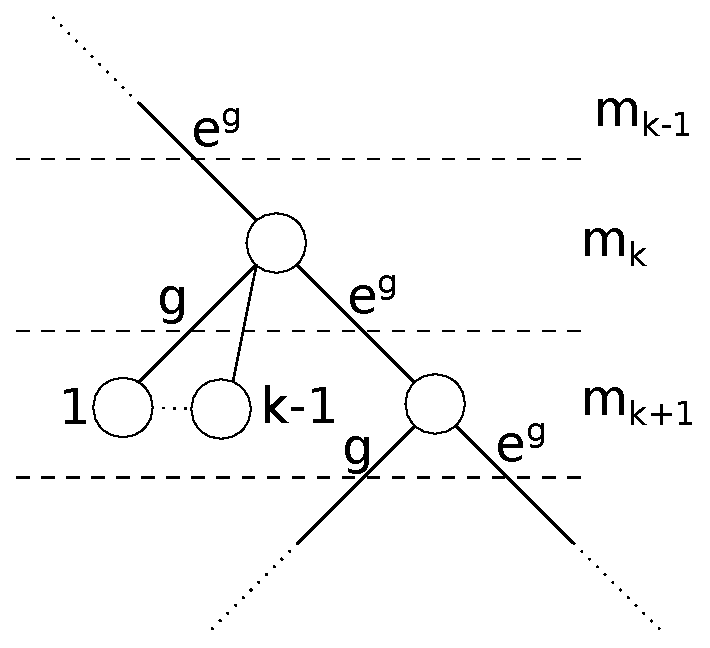
\includegraphics[width = 0.5\textwidth]{./Images/deriv_graph.eps}
	\caption{Illustration of the differentiation scheme.}
	\label{fig:deriv_graph}
\end{figure}

The tree starts with $e^{g}$ at the very top. From there, the derivatives produce a series of terms, one with derivatives of $e^{g}$ and the rest with derivatives of the already present derivatives of $g$. The two are represented by steps to the left and right down the tree. Moving down the tree corresponds to starting with some term, represented by a node, and following the term generated by differentiating a particular factor in that term. In the figure we see a path that has thus far only included steps to the right, and therefore contains $k - 1$ factors of derivatives of $g$, as well as $e^{g}$. We therefore have $k - 1$ left nodes corresponding to terms with derivatives of´ these factors, as well as a right node corresponding to the term which has an extra derivative of $g$. As we have seen above, steps to the left after steps to the right produces correlation functions as factors, meaning that each left node in the figure has a correlation function as a factor - in this particular case factors $\overline{\Psi_{m_{k}}\Psi_{m_{n}}}$ for all $n < k$. Note that this implies that each of these $k - 1$ have $k - 2$ left nodes, and thus that the upper most node and all nodes that are preceded by an equal amount of left and right steps have no left nodes. Because the first derivatives of $g$ are zero, the only contributions to the desired correlation function are found by considering valid paths with an equal number of steps to the right and left.

More explicitly, we are studying
\begin{align*}
	\overline{\Psi_{m_{1}}\dots\Psi_{m_{2N}}} = \eval{\left(\prod\limits_{k = 1}^{2N}\del{}{j_{m_{k}}}\right)e^{g}}_{j = 0} = \eval{\left(\prod\limits_{k = 2N}^{1}\del{}{j_{m_{k}}}\right)e^{g}}_{j = 0},
\end{align*}
where the latter simply denotes a reversal of order for convenience. The term corresponding to the uppermost node in figure \ref{fig:deriv_graph} is equal to
\begin{align*}
	e^{g}\prod\limits_{a = 1}^{k - 1}\left(\frac{1}{2}(B_{m_{a}b} + B_{bm_{a}})j_{b}\right),
\end{align*}
where we use $B = A^{-1}$ for brevity. We now want to consider a step to the left. Stepping to node $n$ from the left we get the term
\begin{align*}
	e^{g}\left(\del{}{j_{m_{k}}}\frac{1}{2}(B_{m_{n}b} + B_{bm_{n}})j_{b}\right)\prod\limits_{a = 1,\ a \neq n}^{k - 1}\left(\frac{1}{2}(B_{m_{a}b} + B_{bm_{a}})j_{b}\right) &= \frac{1}{2}(B_{m_{n}m_{k}} + B_{m_{k}m_{n}})e^{g}\prod\limits_{a = 1,\ a \neq n}^{k - 1}\left(\frac{1}{2}(B_{m_{a}b} + B_{bm_{a}})j_{b}\right) \\
	&= B_{m_{n}m_{k}}e^{g}\prod\limits_{a = 1,\ a \neq n}^{k - 1}\left(\frac{1}{2}(B_{m_{a}b} + B_{bm_{a}})j_{b}\right) \\
	&= \overline{\Psi_{m_{n}}\Psi_{m_{k}}}e^{g}\prod\limits_{a = 1,\ a \neq n}^{k - 1}\left(\frac{1}{2}(B_{m_{a}b} + B_{bm_{a}})j_{b}\right).
\end{align*}
From this we first note the recursive structure of the tree, as the result of taking a step left is an expectation value and a function similar to the one we started with. The effect of taking a specific step to the left after a given number of steps to the right is thus to pick out a particular expectation value.

We may now use the structure of the diagram to infer the value of the desired expectation value. We note that the combination of the first step left and the second step right produces the correlation function $\overline{\Psi_{m_{1}}\Psi_{m_{2}}}$ and returning us to square one. Alternating between left and right thus pairs the $\Psi_{i}$ in order. Taking two steps right before the first step left instead produces two terms with factors $\overline{\Psi_{m_{1}}\Psi_{m_{3}}}$ and $\overline{\Psi_{m_{2}}\Psi_{m_{3}}}$ while leaving a factor. Another step left pairs the remaining $\Psi_{m}$ with $\Psi_{m_{4}}$. For $N = 2$ there are three valid paths, which are the ones discussed above. They combine to form the statement of Wick's theorem for $N = 2$. Repeating this argument for a larger structure, we find that in these paths, all possible pairings of $\Psi_{m}$ are found exactly once, yielding
\begin{align*}
	\overline{\Psi_{i_{1}}\dots\Psi_{i_{2N}}} = \sum\limits_{\text{pairs}}\overline{\Psi_{i_{k_{1}}}\Psi_{i_{k_{2}}}}\dots\overline{\Psi_{i_{k_{2N - 1}}}\Psi_{i_{k_{2N}}}}.
\end{align*}

The complex case carries many similarities to the real case, so this will only be a repetition of the important details. First, we will have to use the probability distribution
\begin{align*}
	P(\Psi) = Ce^{-\Psi\adj A\Psi},
\end{align*}
where $A$ is a Hermitian matrix. Computations with this distribution involves integration over the complex plane for each components. Letting $a$ and $b$ be the real and imaginary of some particular component $\psi$, integration over the complex plain maps onto integration over real space parametrized by $a$ and $b$. We may now introduce independent variables $\psi = a + bi$ and $\psi\cc = a - bi$, which correspond to a rotation in $ab$-space, and integrate over these instead. We thus write the integral as an integral over $\dd{\Psi}\dd{\Psi\adj}$. Similarly to the real case, integration can be carried out by a change of variables specified by the unitary matrix $U$ that diagonalizes $A$.

To extract expectation values, we use the function
\begin{align*}
	F(v, w\adj) = \integ{}{}{\Psi}{\integ{}{}{\Psi\adj}{Ce^{-\Psi\adj A\Psi}e^{w\adj\Psi}e^{\Psi\adj v}}}.
\end{align*}
We introduce shifted variables to find
\begin{align*}
	F(v, w\adj) &= \integ{}{}{\Psi}{\integ{}{}{\Psi\adj}{Ce^{-(\Psi\adj + w\adj W\adj)A(\Psi + Vv)}e^{w\adj(\Psi + Vv)}e^{(\Psi\adj + w\adj W\adj)v}}} \\
	        &= e^{w\adj Vv+ w\adj W\adj v - w\adj W\adj AVv}\integ{}{}{\Psi}{\integ{}{}{\Psi\adj}{Ce^{-\Psi\adj A\Psi - \Psi\adj AVv - w\adj W\adj A\Psi + w\adj\Psi + \Psi\adj v}}}.
\end{align*}
Choosing $W\adj = V = A^{-1}$ we find
\begin{align*}
	F(v, w\adj) &= e^{w\adj A^{-1}v + w\adj A^{-1}v - w\adj A^{-1}v}\integ{}{}{\Psi}{\integ{}{}{\Psi\adj}{Ce^{-\Psi\adj A^{-1}\Psi - \Psi\adj v - w\adj \Psi + w\adj\Psi + \Psi\adj v}}} \\
	        &= e^{w\adj A^{-1}v}\integ{}{}{\Psi}{\integ{}{}{\Psi\adj}{Ce^{-\Psi\adj A^{-1}\Psi}}} \\
	        &= e^{w\adj A^{-1}v}.
\end{align*}
By its definition, we have
\begin{align*}
	\eval{\del{}{v_{i}}F}_{w, v = 0} = \integ{}{}{\Psi}{\integ{}{}{\Psi\adj}{\Psi_{i}\cc Ce^{-\Psi\adj A\Psi}}} = \overline{\Psi_{i}\cc},\ \eval{\del{}{w_{i}}F}_{v, w = 0} = \integ{}{}{\Psi}{\integ{}{}{\Psi\adj}{\Psi_{i}Ce^{-\Psi\adj A\Psi}}} = \overline{\Psi_{i}},
\end{align*}
and similarly for higher-order expectation values. Note the suppression of the adjointness of $w$. In particular we may repeat the arguments for the real case by writing $F$ as $e^{g}$ for $g = w\adj A^{-1}v$. As $g$ is linear in $w$ and $v$, we must have $\overline{\Psi_{i}\Psi_{j}} = \overline{\Psi_{i}\cc\Psi_{j}\cc} = 0$. Finally we find
\begin{align*}
	\overline{\Psi_{i}\Psi_{j}\cc} &= \eval{\del{}{v_{j}}\del{}{w_{i}}F}_{v, w = 0} \\
	                               &= \eval{\del{}{v_{j}}\left((A)^{-1}_{ik}v_{k}e^{g}\right)}_{v, w = 0} \\
	                               &= \eval{(A)^{-1}_{ij}e^{g}}_{v, w = 0} \\
	                               &= (A)^{-1}_{ij}.
\end{align*}

The argument for higher-order correlation functions used in the real case may also be applied to the complex case. As we see from the above, it is in fact even simpler. By writing
\begin{align*}
	\overline{\Psi_{i_{1}}\dots\Psi_{i_{N}}\Psi_{j_{1}}\cc\dots\Psi_{j_{N}}\cc} = \eval{\left(\prod\limits_{n = 1}^{N}\del{}{v_{j_{n}}}\right)\left(\prod\limits_{m = 1}^{N}\del{}{w_{i_{m}}}\right)F}_{v, w = 0},
\end{align*}
we note that $g$ being linear in both $v$ and $w$ implies that the first $N$ layers of the tree contain only right steps. As $g = 0$ for either $v$ or $w$ equal to zero, there must still be a balance between right and left steps, meaning that we only need to consider left steps in the lower half of the tree. In similar fashion to the real case, the first step to the left creates $N$ nodes, each with a factor $\overline{\Psi_{i_{1}}\Psi_{j_{k}}\cc}$ for some $k$ unique to that node in that particular level. Similar pairings occur down through the structure, and the final result is
\begin{align*}
	\overline{\Psi_{i_{1}}\cc\dots\Psi_{i_{N}}\cc\Psi_{j_{1}}\dots\Psi_{j_{N}}} = \sum\limits_{P(1, \dots, N)}\overline{\Psi_{i_{P(1)}}\Psi_{j_{1}}}\ \overline{\Psi_{i_{P(2)}}\Psi_{j_{2}}}\dots\overline{\Psi_{i_{P(N)}}\Psi_{j_{N}}}.
\end{align*}